\begin{comment}
\begin{figure}
\centering
	% To include a figure from a file named example.*
	% Allowable file formats are eps or ps if compiling using latex
	% or pdf, png, jpg if compiling using pdflatex
	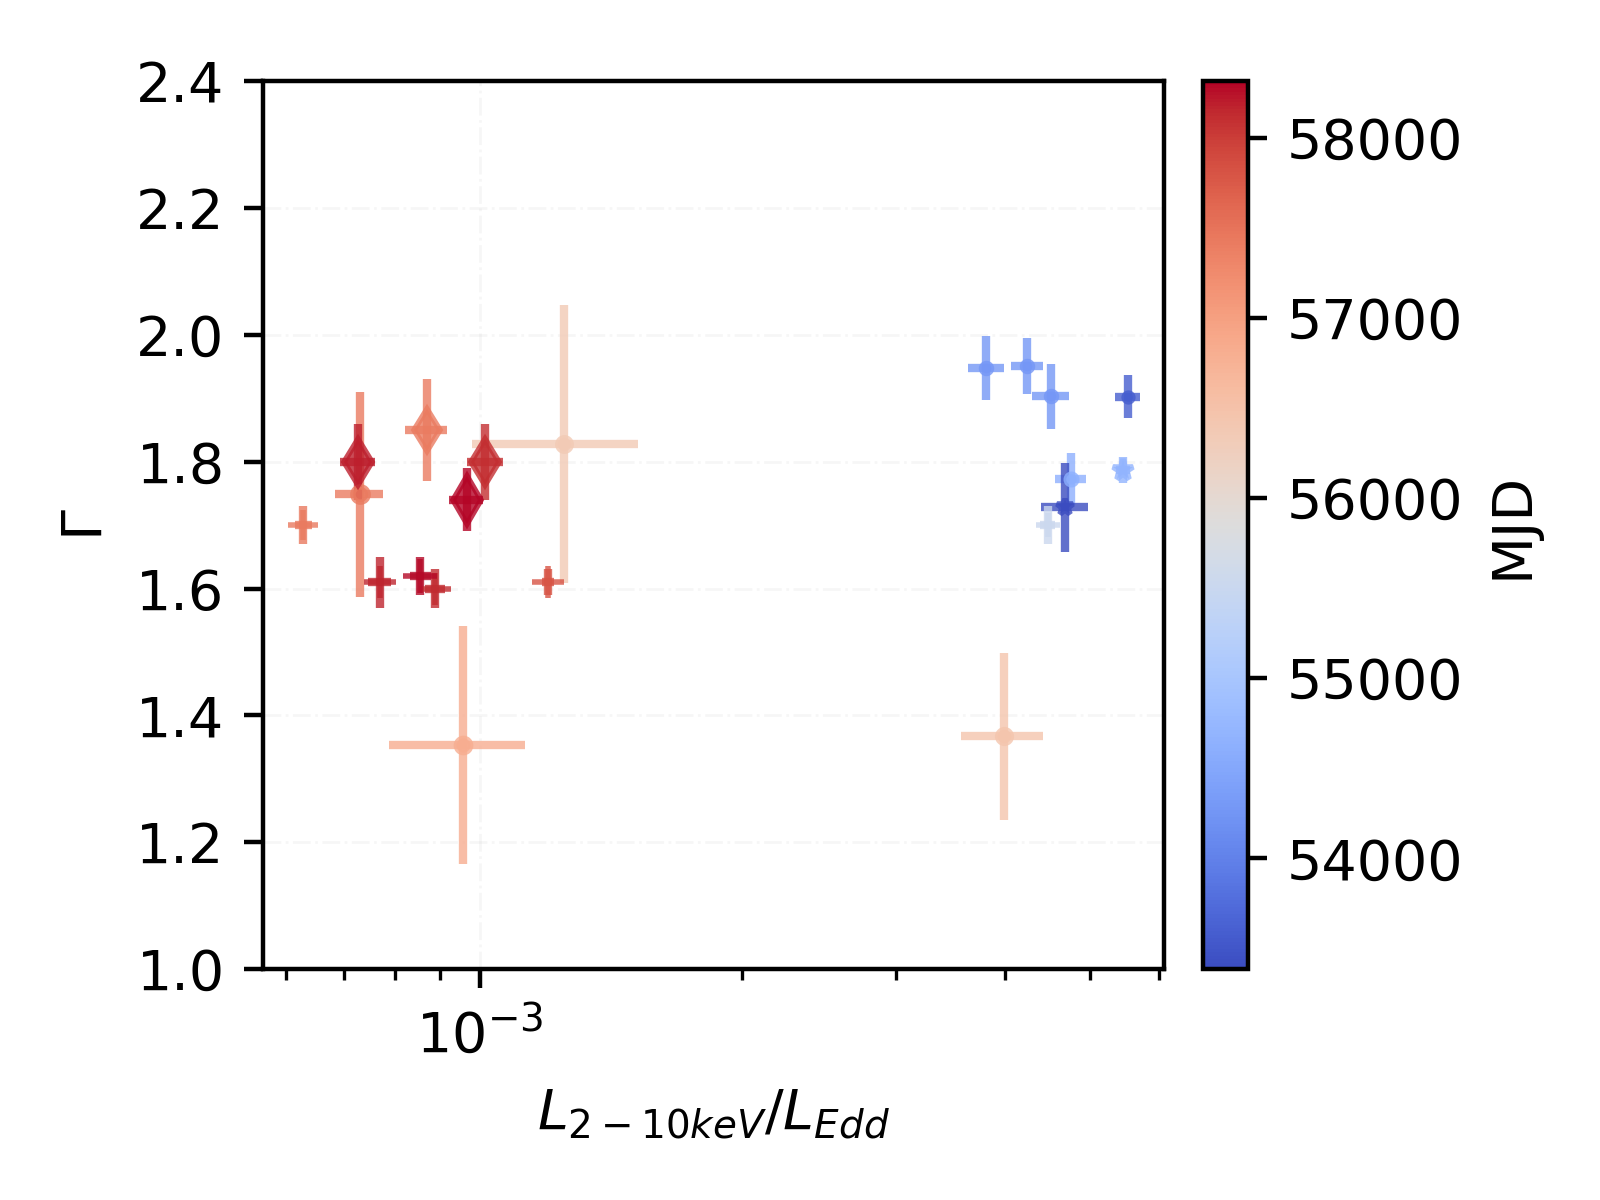
\includegraphics[width=0.7\columnwidth]{./pic/xrayappendgood-eddrate-g-tmap.png}
    \caption{$\Gamma$ and eddington rate evolution}
    \label{fig:xrayappendgood-eddrate-g-tmap}
\end{figure}
\end{comment}


\citet{1997MNRAS.286..513R} analysed X-ray spectrum of 24 type 1 AGN sampled from the EXOSAT survey of \citet{1989MNRAS.240..833T} and the Ginga survey of \citet{1994MNRAS.268..405N} with 18 Seyfert 1 galaxies and 2 radio-quiet quasars, the others are 3 broad-line radio galaxies and 1 radio-loud quasar. The X-ray spectrum fit based on power-law continuum, Gaussian line, two absorption edges, plus intrinsic and Galactic absorption shows a random distribution in $\Gamma-L_x$ diagram with Spearman's correlation coefficient: 0.25, pvalue: 0.24 and Pearson's correlation coefficient: -0.14, pvalue: 0.52, where the luminosity range from $1.78\times 10^{41}$ to $1.53\times 10^{47} erg s^{-1}$. It is consistent with \citet{2015AASP....5...79S} sampled from 97 Seyfert 1 galaxies, where the luminosity range from $4.5\times 10^{41}$ to $9\times 10^{44} erg s^{-1}$. 


\citet{2008ApJ...682...81S} found the positive correlation between the hard X-ray photon index ($\Gamma$) and accretion rate (L/LEdd) for 35 moderate to high luminosity Radio-Quiet AGNs with z at 1.3$\sim$3.2. They also found that the optical-X-ray spectral slope ($\alpha_{OX}$) depends mainly on optical-UV luminosity, rather than $L/L_{Edd}$, consistent with \citet{2012MNRAS.423..600S} but in Type 1 AGNs at low z(0.005$\sim$0.31) where luminosity mainly drives the X-ray to UV emission ratio , rather than $M_{BH}$ or $L/L_{Edd}$.

\citet{2008AJ....135.1505S} showed strong and positive $\Gamma-L_x$ correlation in 173 bright radio-quiet active galactic nuclei (AGNs) in the redshift range 0.1$\sim$4 when type I and no-type I AGNs are divided into sub-samples with luminosity range from $10^{42}$ to $10^{45} erg s^{-1}$.



\citet{2014MNRAS.443...72J,2015MNRAS.447.1692Y} found the anti-correlation of $\Gamma-L_x/L_{Edd}$ in low-accreting AGNs with $10^{-10}\leq L_x/L_{Edd} \leq 10^{-3}$ and $10^{-6.5}\leq L_x/L_{Edd} \leq 10^{-3}$, respectively, while positive correlation of $\Gamma-L_x/L_{Edd}$ was found when $L_x/L_{Edd} \geq 10^{-3}$ in \citet{2015MNRAS.447.1692Y}.





\citet{2017ApJ...841L..18M} summarized that as X-ray luminosity increase, the relative fraction of observed Type 2 AGN to Type 1 AGN decreased, even though the median X-ray luminosity is almost equal, where only AGNs with $L_x \geq 10^{42} erg s^{-1}$ and $z \leq 1$ were considered to avoid the host galaxy contamination and evolution effects.

\citet{2018MNRAS.476L..34S} modeled the AGN variability timescale from days to Gyr.

\citet{2019arXiv190800742C} reviewed the basic scenarios where the Broad Line Region (BLR) originate, such as inflow model, formation 'in situ', wind-disk model, etc. 


The luminosity of AGN might drive the emission line and disk-corona in separate ways.



\begin{figure}
\centering
	% To include a figure from a file named example.*
	% Allowable file formats are eps or ps if compiling using latex
	% or pdf, png, jpg if compiling using pdflatex
	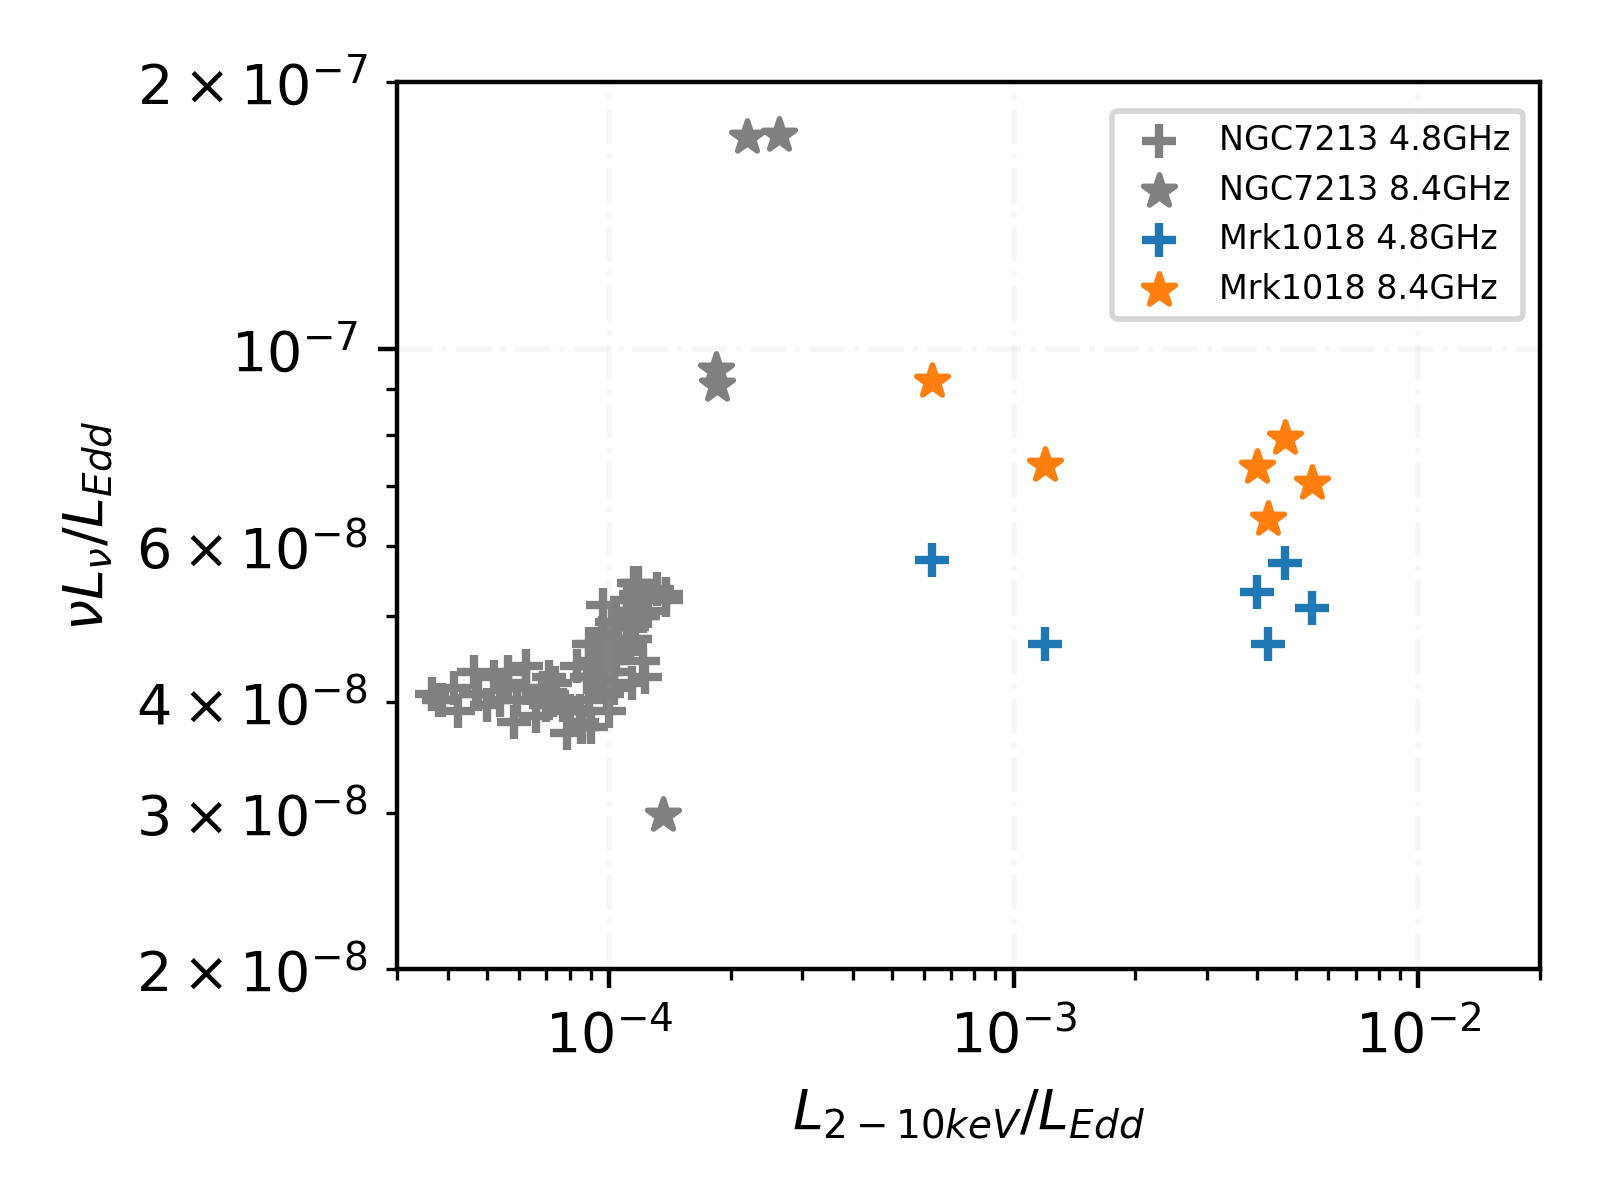
\includegraphics[width=0.9\textwidth]{./pic/Mrk1018_ngc7213_radio_xray_rate.png}
    \caption{Quasi-simultaneous $\nu L_{\nu}/L_{Edd}-L_{2-10keV}/L_{Edd}$ relation of Mrk1018}
    \label{fig:radio-xray-rate_relation_plus_ngc7213}
\end{figure}


\begin{figure}
\centering
	% To include a figure from a file named example.*
	% Allowable file formats are eps or ps if compiling using latex
	% or pdf, png, jpg if compiling using pdflatex
	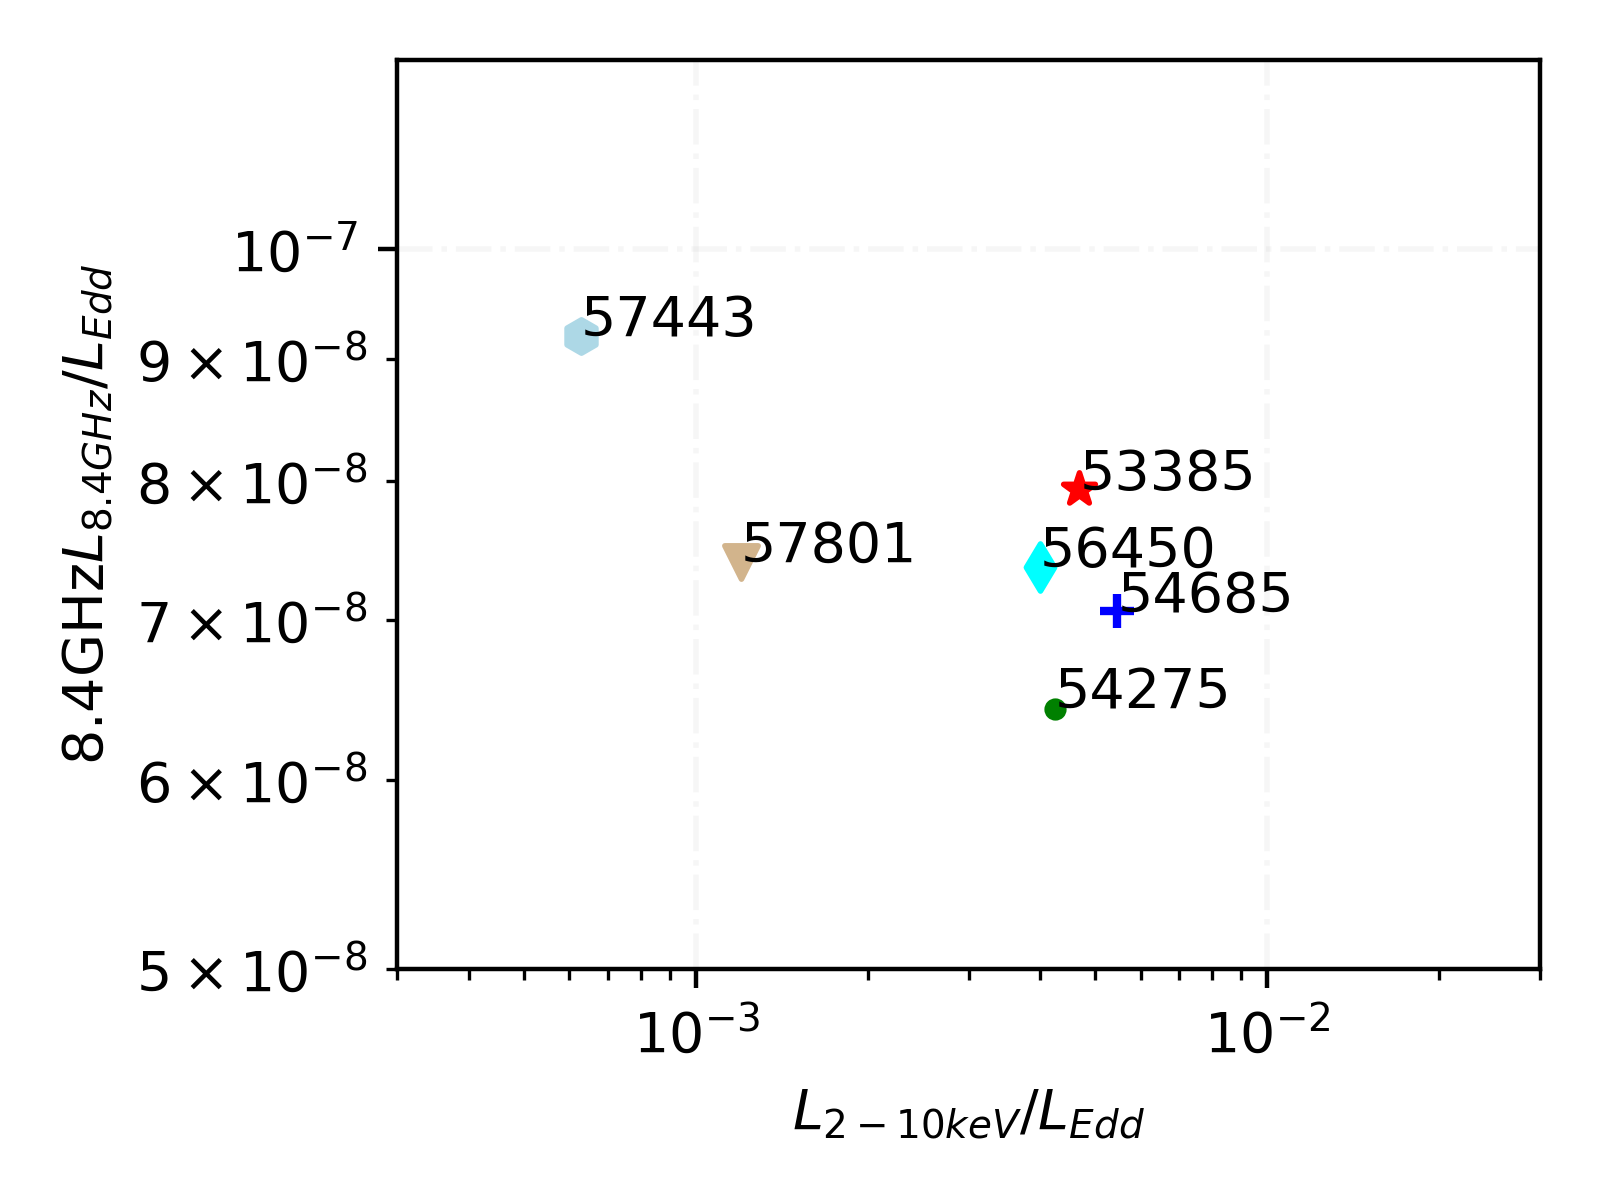
\includegraphics[width=0.9\textwidth]{./pic/Mrk1018_radio_xray_sel1_rate.png}
    \caption{Quasi-simultaneous $\nu L_{\nu}/L_{Edd}-L_{2-10keV}/L_{Edd}$ relation of Mrk1018}
    \label{fig:radio-xray-relation}
\end{figure}